


\part{Extendiendo el Simulador simusched}

\section{Ejercicio 3}

Completamos la implementaci\'on del scheduler Round-Robin implementando los todos de la clase SchedRR.

Este scheduler recibe en quantum y permite a cada tarea ejecutar como maximo ese tiempo, una vez finalizado ese tiempo continua con la siguiente tarea lista para ejecutar.

Ver resoluci\'on en los archivos \verb|sched rr.cpp| y \verb|sched rr.h|.

\section{Ejercicio 4}

Realizamos dos lotes de prueba para observar el comportamiento de del scheduler Round-Robin.

Para tal fin creamos el tipo de Tarea TaskCPUIOCPU que recibe 3 parametros:

\begin{enumerate}
 \item n Tiempo de ejecuci\'on de CPU en ciclos de reloj
 \item i Tiempo de ejecuci\'on de IO en ciclos de reloj
 \item m Tiempo de ejecuci\'on de CPU en ciclos de reloj
\end{enumerate}

Esta tarea ejecuta en el CPU (n) se bloquea por (i) y luego sigue ejecutando (m).

\subsection{Lote 1}

Creamos el siguiente grupo de tareas \verb|ejercicio4_1.tsk|

\begin{framed}
\begin{verbatim}
# FILE ejercicio4_1.tsk
*2 TaskCPU 30
TaskCPUIOCPU 10 20 10
\end{verbatim}
\end{framed}

Luego ejecutamos Simusched con los siguientes parametros:

\begin{framed}
\begin{verbatim}
./simusched ejercicio4_1.tsk 1 SchedRR 3 | python graphsched.py > ejercicio4_1.png
\end{verbatim}
\end{framed}

\begin{figure}[h!]
  \caption{Dos tareas de uso intensivo de CPU y una tarea de tipo TaskCPUIOCPU.}
  \centering
    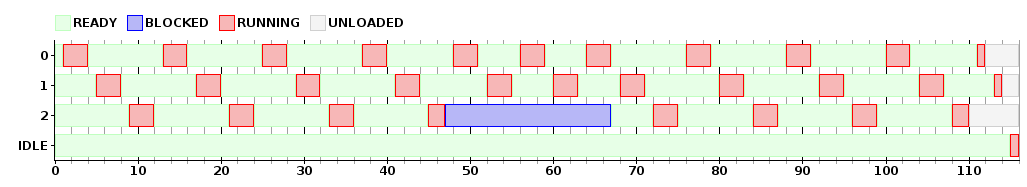
\includegraphics[width=1\textwidth]{img/ejercicio4_1.png}
\end{figure}

Se puede ver en el grafico que se van alternando los 3 procesos con un quantum de 3 unidades hasta que el proceso (2) se bloquea.

Mientras el (2) est\'a bloqueado se puede ver que los otros dos procesos van altenando su ejecuci\'on. 

Hasta que el proceso (2) se desblquea y nuevamente se vuelven a alternar los 3 procesos.

\subsection{Lote 2}

Utilizamos nuevamente la tarea que creamos anteriormente TaskCPUIOCPU.

Creamos el archivo \verb|ejercicio4_2.tsk|

\begin{framed}
\begin{verbatim}
# FILE ejercicio4_2.tsk
TaskCPUIOCPU 10 20 10
@3
TaskCPUIOCPU 15 20 5
@10
TaskCPU 10
\end{verbatim}
\end{framed}

Luego ejecutamos Simusched con los siguientes parametros:

\begin{framed}
\begin{verbatim}
./simusched ejercicio4_2.tsk 1 SchedRR 4 | python graphsched.py > ejercicio4_2.png
\end{verbatim}
\end{framed}

\begin{figure}[h!]
  \caption{Dos tareas de tipo TaskCPUIOCPU y una tarea de uso intensivo de CPU.}
  \centering
    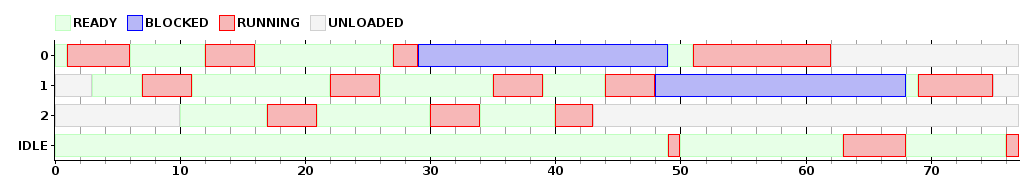
\includegraphics[width=1\textwidth]{img/ejercicio4_2.png}
\end{figure}

Se ve en el grafico que se carga la tarea 0 y se comienza a ejecutar por el quantum de 4.

Luego, cuando esta finaliza la tarea 1 ya est\'a en la cola de listos, por lo que comienza a ejecutar hasta finalizar su quantum.

Para ese momento las tareas 0 y 2 estan en la cola de listos, por lo que comienza a ejecutar la 0 que estaba en primer lugar.

Despues de eso las tres tareas ya se encuentran cargadas y se van ejecutando hasta finalizar su quantum hasta que el ciclo 29 la tarea 0 se bloquea.

Por lo que siguen ejecutando las tareas 1 y 2 hasta que el el ciclo 43 la tarea 2 finaliza, y en el ciclo 48 la tarea 1 se bloquea, por lo que el procesador queda ocioso.

En el ciclo 49 la tarea 0 finaliza su entrada/salida, por lo que continua su ejecucion. 

En el ciclo 62 la tarea 0 finaliza y el procesador queda nuevamente ocioso.

En el ciclo 68 la tarea 1 finaliza su entrada/salida y ejecuta hasta finalizar.


\section{Ejercicio 5}

Completamos la implementaci\'on del scheduler Multilevel Feedback Queue implementando los todos de la clase SchedMFQ.

Este scheduler utiliza n colas con Round-Robin, y recibe como parametro el quantum de cada una de las colas.

Ver resoluci\'on en los archivos \verb|sched mfq.cpp| y \verb|sched mfq.h|.
